\documentclass[fleqn]{article}

\usepackage[margin=1in]{geometry}
\usepackage{amsfonts,amsmath,amssymb}
\usepackage{fancyhdr}
\usepackage{lastpage}
\usepackage{tcolorbox}
\usepackage{graphicx}
\usepackage{xcolor}
\usepackage{url}
\usepackage[hidelinks]{hyperref}
\usepackage{titlesec}
\usepackage{parskip}
\usepackage{tikz}
\usepackage{listings}
\tcbuselibrary{listings}  % Requires both listings + tcolorbox
% Color definitions
\usepackage{tabularx}
\definecolor{codegray}{gray}{0.95}
\definecolor{commentgreen}{rgb}{0,0.6,0}
\definecolor{keywordblue}{rgb}{0.25,0.35,0.75}

% Python style
\lstdefinestyle{mypython}{
    backgroundcolor=\color{codegray},
    commentstyle=\color{commentgreen}\ttfamily\normalsize,
    keywordstyle=\color{keywordblue}\bfseries,
    stringstyle=\color{red!60!black},
    numberstyle=\small\color{gray},
    basicstyle=\ttfamily\normalsize,
    breaklines=true,
    frame=single,
    numbers=left,
    numbersep=5pt,
    showstringspaces=false,
    tabsize=4,
    language=Python,
    columns=fullflexible, % Fixes whitespace collapse
    keepspaces=true      % Preserves spaces in code
}

% ---------------------------------------------------------------------------------------------------
% Template values
\newcommand{\myLogo}{LaTeX project photo}
\newcommand{\myName}{Aryan Burnwal}
\newcommand{\myJobTitle}{Student, B.tech}
\newcommand{\myLocation}{India}
\newcommand{\myURL}{www.linkedin.com/in/aryan-burnwal-21a622253}
\newcommand{\mygithub}{github.com/Arihant-3}
\newcommand{\myEmail}{work.aburnwal@gmail.com}
\newcommand{\myAssignment}{Project: DSA-less Problems}
\newcommand{\mydate}{14, April to 14, May 2025}

% Macro for custom title page signature header
\newsavebox{\myTitleSignature}
\sbox{\myTitleSignature}{%
\begin{tabularx}{\textwidth}{@{}l X@{}}
\begin{minipage}[c][5pt][c]{\hsize}
  \raggedright\textbf{\myName} \\
  {\small \myJobTitle} \\
  {\small \myLocation} \\
  {\small \url{https://\myURL}} \\
  {\small \url{https://\mygithub}} \\
  {\small \href{mailto:\myEmail}{\myEmail}}
\end{minipage}
&
\begin{minipage}[c][1.5in][c]{\hsize}
  \centering
  \includegraphics[height=1.5in]{\myLogo}
\end{minipage}
\end{tabularx}
}

% --------------------------------------------------------------------------------------------------

\pagestyle{fancy}
\lhead{30 Day Problem Challenge}
\chead{}
\rhead{AB}
\lfoot{}
\cfoot{Page : \thepage }
\rfoot{}


\titleformat{\section}{\large\bfseries}{}{0em}{}
\titleformat{\subsection}{\normalsize\bfseries}{}{0em}{}

\setlength{\parindent}{0pt}
\linespread{1.1}

% Answer box command
\newcommand{\problemAnswer}[1]{%
\begin{tcolorbox}[
  colback=gray!10!white,
  title=,
  listing only,
  listing options={style=mypython}
]
\large
#1 % Python code goes here
\end{tcolorbox}
}

% For dotted lines
\newcommand{\daySeparator}{
    \vspace{1cm}
    \begin{center}
        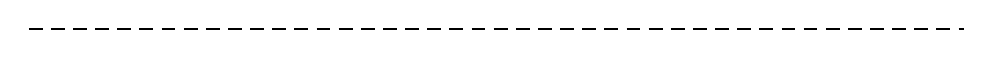
\begin{tikzpicture}
            \draw[dash pattern=on 5pt off 3pt, thick] (0,0) -- (0.98\linewidth,0);
        \end{tikzpicture}
    \end{center}
    \vspace{1cm}
}

% Custom command for unnumbered sections
\newcommand{\mysection}[1]{%
  \section*{\texorpdfstring{$\underrightarrow{\text{#1}}$}{#1}}%
  \phantomsection%
  \addcontentsline{toc}{section}{#1}%
}

% Custom command for unnumbered subsections
\newcommand{\mysubsection}[1]{%
  \subsection*{#1}%
  \phantomsection%
  \addcontentsline{toc}{subsection}{#1}%
}

% ---------------------------------------------------------------------------------------------------
% ---------------------------------------------------------------------------------------------------

\begin{document}

\thispagestyle{empty} 
% Use custom title macro instead
\usebox{\myTitleSignature}
\vspace{1.5cm} % spacing below title header

\begin{center}
    {\Huge \textbf{The Thinking Path – \\ Powered by Logic, Framed in LaTeX}}\\[1ex]
    \rule{6.5in}{0.9pt}\\
    {\small \textbf{A documentation of problem-solving through logic, mathematics, and structured thinking—without leaning on data structures.}}\\[0.5ex]
    \rule{6.5in}{0.9pt}\\
    \textit{By Aryan Burnwal}\\
    Timeline: 14 April – 14 May, 2025
\end{center}

\vspace{1.2cm}

\setcounter{tocdepth}{2} % Include up to subsections in ToC
\tableofcontents
\newpage

% -------------------------------
\mysection{Day 1}
% -------------------------------

\mysubsection{The Problem Statement :-}
\problemAnswer{
Given an integer \colorbox{gray!20}{$n$}, find the number of trailing zeros in \colorbox{gray!20}{$n!$} (i.e., \colorbox{gray!20}{$n$} factorial).
}

\problemAnswer{
\subsubsection*{(i) Constraints}
$-$ \colorbox{gray!20}{$1 \leq n \leq 10^9$}  \\
$-$ You are \textbf{not allowed} to compute the actual factorial!
\vspace{0.5em}
\subsubsection*{(ii) Hints:}
$-$ Where do trailing zeros in numbers come from? \\
$-$ What factor(s) in multiplication create zeros at the end? \\
$-$ Can you spot a pattern or rule? 
}

\mysubsection{1. My Thought Process}
\problemAnswer{
$-$ First, I started thinking about how zeros are formed at the end of a number. I realized that every zero at the end comes from a 10, and 10 is made from multiplying 2 and 5. Since there are usually more 2s than 5s in factorials, the number of 5s basically decides how many zeros we get. 
\vspace*{0.2cm} \\
$-$ So, I thought: how often does a 5 appear in the factorial? Every time we have a multiple of 5, we get one 5. That means for every 5 numbers, we gain one trailing zero. But then I noticed something more-numbers like 25 (which is $5^2$), 125 (which is $5^3$), etc., contribute more than one 5. So we have to count those extra times too.
\vspace*{0.2cm} \\
$-$ That’s when I realized the trick is to divide n by 5, then again by 25, then by 125, and so on. Each time we divide and take the floor value, it tells us how many extra 5s are hiding in those powers. This gives the total number of zeros at the end.
}

\mysubsection{2. The Solution}
\problemAnswer{
\large{Trailing Zeros in $ n! $ =} 
\Large{$\left\lfloor \frac{n}{5} \right\rfloor + \left\lfloor \frac{n}{25} \right\rfloor + \left\lfloor \frac{n}{125} \right\rfloor + \left\lfloor \frac{n}{625} \right\rfloor \cdots$}
}

\mysubsection{3. Actual Intuition}
\problemAnswer{
$\cdot$ A trailing zero is created by multiplying a \textbf{2 × 5}. \\
$\cdot$ In \colorbox{gray!20}{$n!$}, there are \textbf{more 2s than 5s}. \\
$\cdot$ So, we count how many times \textbf{5 is a factor} in all numbers from 1 to n. \\
But we also need to include \textbf{25, 125, 625, ...} because numbers like 25 give \textbf{two 5s}, 125 gives \textbf{three 5s}, etc.
}

\daySeparator

% -------------------------------
\mysection{Day 2}
% -------------------------------

\mysubsection{The Problem Statement :-}
\problemAnswer{
Given a non-negative integer \colorbox{gray!20}{$n$}, repeatedly add its digits until the result has only one digit. \\
Return that final one-digit number.
}

\problemAnswer{
\subsubsection*{(i) Constraints:}
$-$ \colorbox{gray!20}{$0 \leq n \leq 2 \times 10^9$}  \\
$-$ Try to solve this \textbf{without loops or recursion} if possible.
\vspace{0.5em}
\subsubsection*{(ii) Hints:}
$-$ Is there a \textbf{mathematical pattern} in digital root? \\
$-$ Can you find a shortcut?
}

\mysubsection{1. The Solution}
\problemAnswer{
\begin{large}
    If $n=0$, then $result=0$; else, $result=1+((n-1) \, mod \, 9)$
\end{large}
}

\mysubsection{2. Actual Intuition}
\problemAnswer{
This is based on a cool math fact called \textbf{“mod 9 congruence”} - the sum of digits of any number is \textbf{congruent to the number itself modulo 9}.
\vspace*{0.2cm} \\
So instead of looping and summing digits again and again, you can just do:
Digital Root of $n=1+((n-1)  mod  9)$
}

\daySeparator

% -------------------------------
\mysection{Day 3}
% -------------------------------

\mysubsection{The Problem Statement :-}
\problemAnswer{
A monkey is trying to climb a tree of height \colorbox{gray!20}{H} meters. \\
Each day it climbs up \colorbox{gray!20}{U} meters, but every night it slips down \colorbox{gray!20}{D} meters. \\
After how many days will the monkey reach or exceed the top of the tree?
\vspace{3pt}

$\bullet$ Inputs:

\colorbox{gray!20}{H}: Total height of the tree. \\
\colorbox{gray!20}{U}: Distance the monkey climbs during the day. \\
\colorbox{gray!20}{D}: Distance the monkey slides down at night. 
\vspace{3pt}

$\bullet$ Output:
Return the \textbf{number of days} it takes to reach the top.
}

\problemAnswer{
\subsubsection*{(i) Constraints:}
$-$ The monkey \textbf{doesn’t slide back} on the \textbf{final day} if it reaches or exceeds the height during the day.  \\
$-$ \colorbox{gray!20}{$ 1 \leq D < U \leq H \leq 10^9 $}
\vspace{0.5em}
\subsubsection*{(ii) Hints:}
$-$ Can you find a formula instead of simulating day by day? \\
$-$ Is there a way to calculate how many \textbf{full cycles} the monkey needs before the final climb?
}

\mysubsection{1. My Thought Process}
\problemAnswer{
$i)$ Let’s say it takes the monkey x days to reach the top of the tree. \\
$ii)$ On the last day, the monkey climbs up and reaches the top during the day, so it doesn’t slide back at night. \\
$iii)$ This means for the first (x - 1) days, the monkey climbs during the day and slides back at night-so the net progress per day is (U-D) meters. \\
$iv)$ By the end of the (x-1) days, the monkey must be close enough to the top that one final climb of U meters will get it to or past the height H. \\
$v)$ So, the total distance that needs to be covered in the first (x-1) days is (H-U). \\
$vi)$ This gives the equation: 
\begin{center}
    $(x-1) \times (U-D)=H-U$
\end{center}
$vii)$ From here, we can solve for x.
}

\mysubsection{2. The Solution}
\problemAnswer{
\begin{Large}days=\( \left\lceil\frac{H-U}{U-D} \right\rceil+1 \)\end{Large}
}

\daySeparator

% -------------------------------
\mysection{Day 4}
% -------------------------------

\mysubsection{The Problem Statement :-}
\problemAnswer{
You have \colorbox{gray!20}{$n$} bulbs, all turned \textbf{off} initially.\\
You make \colorbox{gray!20}{$n$} passes over them.\\
$\cdot$ \textbf{On the 1st pass, you toggle every bulb (turn it on).}\\
$\cdot$ \textbf{On the 2nd pass, you toggle every 2nd bulb.}\\
$\cdot$ \textbf{On the 3rd pass, you toggle every 3rd bulb.}\\
$\cdot$ \, '$\cdots$'\\
$\cdot$ \textbf{On the \colorbox{gray!20}{i-th} pass, you toggle every i-th bulb.}
\vspace*{0.2cm}

After \colorbox{gray!20}{n} passes, how many bulbs are \textbf{on}?
}

\problemAnswer{
\subsubsection*{Hints:}
$-$ When does a bulb end up ON after all toggles? \\
$-$ Try small cases: n = 1 to 10 \\
$-$ Look for a pattern in which positions remain ON.
}

\mysubsection{1. My Thought Process}
\problemAnswer{
$i)$ I wasn’t sure of the pattern at first, so I decided to try a brute-force approach. \\
$ii)$ I checked all possible values of n from 1 to 10. \\
$iii)$ For each value, I manually went through the process to see which switches (or bulbs, etc.) were ON and which were OFF at the end. \\
$iv)$ I carefully counted how many were ON and how many were OFF for each n. \\
$v)$ After doing this for a few values, I started noticing a pattern of $\sqrt{5}$ forming based on the positions that remain ON. 
$vi)$ That helped me understand the logic behind the problem better and made it easier to generalize the answer later.
}

\mysubsection{2. The Solution}
\problemAnswer{
\begin{large}Number of bulb that remains \textbf{ON}=\( \left\lfloor \sqrt{n} \right\rfloor \)\end{large}
}

\mysubsection{3. Actual Intuition}
\problemAnswer{
$-$ A bulb is toggled \textbf{once for every divisor} it has. \\
$-$ Most numbers have \textbf{even} number of divisors \textbf{(paired up)}. \\
$-$ But \textbf{perfect squares} have \textbf{odd number of divisors} - because one of the divisors is repeated (like 4 has divisors 1,2,4 - 2 appears only once). \\
$\cdot$ So only \textbf{bulbs at perfect square positions} (1, 4, 9, 16...) will be ON after all passes.
}

\daySeparator

% -------------------------------
\mysection{Day 5}
% -------------------------------

\mysubsection{The Problem Statement :-}
\problemAnswer{
You are given a list of \colorbox{gray!20}{$n$} integers. Every number appears \textbf{exactly twice}, except for \textbf{one number that appears only once}.

Find that \textbf{unique number} in \textbf{O(n)} time and \textbf{O(1)} space.
}

\problemAnswer{
\subsubsection*{(i) Constraints:}
$-$ $1 \leq n \leq 10^6$ \\
$-$ All numbers are non-negative. \\
$-$ Use no extra space like hash maps or sets.
\vspace{0.5em}
\subsubsection*{(ii) Hints:}
$-$ Can you use bitwise operators? \\
$-$ What happens when you XOR a number with itself?
}

\mysubsection{1. The Solution}
\problemAnswer{
\begin{large}
Use : \textbf{XOR}, short for eXclusive OR. \\
$\bullet$ \colorbox{gray!20}{\textasciicircum} is same as \colorbox{gray!20}{$\oplus$} for XOR operation
\end{large}
}

\mysubsection{2. Analysis}
\problemAnswer{
Let’s review the \textbf(key properties) of XOR (\colorbox{gray!20}{$\bigoplus$}): \\
1. \textbf{$a \oplus a = 0$} $\rightarrow$ A number XORed with itself becomes zero.

2. \textbf{$a \oplus  0 = a$} $\rightarrow$ A number XORed with zero stays the same.

3. XOR is \textbf{commutative} and \textbf{associative} :

$\bullet$ \colorbox{gray!20}{$a \oplus b \oplus c = c \oplus b \oplus a$} : Order doesn’t matter.
}

\daySeparator

% -------------------------------
\mysection{Day 6}
% -------------------------------

\mysubsection{The Problem Statement :-}
\problemAnswer{
You have 8 prison cells, each can be occupied (1) or vacant (0), arranged in a row.\\
Each day, the state of the cells changes according to the following rule:\\
$\cdot$ \textbf{A cell becomes 1 (occupied) if its two adjacent neighbors are both occupied or both vacant.}\\
$\cdot$ \textbf{Otherwise, the cell becomes 0.}\\
$\cdot$ \textbf{First and last cells have no two neighbors, so they always become 0 the next day.}\\
Given the initial state and a number \colorbox{gray!20}{$N$}, return the state of the prison after \colorbox{gray!20}{$N$} days.
}

\problemAnswer{
\subsubsection*{(i) Constraints:}
$-$ \colorbox{gray!20}{initial} is a list of length 8, containing only 0s and 1s.\\
$-$ \colorbox{gray!20}{$0 \leq n \leq 10^9$} ← yes, \textbf{1 billion!}
\vspace{0.5em}
\subsubsection*{(ii) Hints:}
$-$ What happens if you simulate it naively? \\
$-$ Do the cell states repeat? If so, can you detect a cycle? \\
$-$ How many unique configurations are even possible?
}

\mysubsection{1. The Solution}
\problemAnswer{
\textbf{Procedures to Solve It:}

1. Simulate day by day, keeping track of seen states. \\
2. Once you see a repeating state, you've found the cycle length. \\
3. Now use modulus: \\
$\cdot$ Instead of simulating all $N$ days, \\
$\cdot$ Do only \colorbox{gray!20}{$N$ \% cycle\_length} days from the start of the cycle!
}
\begin{tcolorbox}[colback=gray!10!white, title=Answer]
\textbf{Pseudocode: }
\begin{lstlisting}[style=mypython]
def prisonAfterNDays(cells, N):
    seen = {}
    while N > 0:
        state = tuple(cells)
        if state in seen:
            cycle_length = seen[state] - N
            N %= cycle_length
        seen[state] = N
        
        N -= 1
        next_cells = [0]  # first cell always 0
        for i in range(1, 7):
            next_cells.append(1 if cells[i-1] == cells[i+1] else 0)
        next_cells.append(0)  # last cell always 0
        cells = next_cells
    return cells
\end{lstlisting}
\end{tcolorbox}

\mysubsection{2. Core Intuition}
\problemAnswer{
$\cdot$ To find the state of the prison cells after \( N \) days, follow these steps: \\
$i)$ Each cell updates daily based on its two adjacent neighbors (left and right). \\
$ii)$ A cell becomes 1 (occupied) if both neighbors are either occupied (1) or both vacant (0). \\
$iii)$ If the neighbors are different, the cell becomes 0 (vacant). \\
$iv)$ The first and last cells always become 0, as they do not have two neighbors. \\
$v)$ Repeat this process for \( N \) days, updating all cells simultaneously each day. \\
$vi)$ Since there are only a limited number of possible states (256), the sequence will eventually enter a cycle (repeat itself). \\
$vii)$ If a cycle is detected, use it to skip ahead: \\
Instead of simulating all \( N \) days, compute \( N \mod \text{cycle\_length} \) and simulate only the remaining steps. \\
This approach ensures correctness and efficiency, even for large values of \( N \).
}

\daySeparator

% -------------------------------
\mysection{Day 7}
% -------------------------------

\mysubsection{The Problem Statement :-}
\problemAnswer{
You’re playing a game with a pile of \colorbox{gray!20}{n} stones. \\
You and your friend take turns removing 1, 2, or 3 stones. \\
The person who removes the \textbf{last stone wins}. \\
You go first. \textbf{Can you guarantee a win} if both play optimally?

\vspace{3pt}
$\bullet$ Inputs:

\colorbox{gray!20}{n}: total number of stones.

\vspace{3pt}
$\bullet$ Output:
Return \colorbox{gray!20}{True} if you can \textbf{guarantee a win}, else \colorbox{gray!20}{False}.
}

\problemAnswer{
\subsubsection*{Hints:}
Try small values of \colorbox{gray!20}{n = 1} to \colorbox{gray!20}{10}, and look for a pattern: \\
$-$ Who wins at \colorbox{gray!20}{n = 1, 2, 3, 4}? \\
$-$ What do the losing positions have in common?
}

\mysubsection{1. My Thought Process}
\problemAnswer{
$i)$ At first, I didn’t know the winning strategy, so I decided to use brute force and try out small values of n. \\
$ii)$ I went from n = 1 to around n = 10 and looked at all possible moves I could make: removing 1, 2, or 3 stones. \\
$iii)$ For each case, I asked myself: \\
\hspace*{5pt} $-$ "If I take 1 stone now, what will my opponent be left with?" \\
\hspace*{5pt} $-$ "Can they win from there if they play optimally?" \\
\hspace*{5pt} $-$ I repeated this for taking 2 and 3 stones too. \\
$iv)$ I noticed that if the number of stones was a multiple of 4, I would always end up losing no matter what I played-because whatever I do, my opponent can always bring it back to a multiple of 4. \\
$v)$ But if it’s not a multiple of 4, I can always make a move that gives my opponent a multiple of 4, putting them in the losing position. \\
$vi)$ So I realized the pattern: \\
\hspace*{5pt} $-$ If n \% 4 == 0, I cannot guarantee a win. \\
\hspace*{5pt} $-$ Otherwise, I can guarantee a win.
}

\mysubsection{2. The Solution}
\problemAnswer{
\begin{large}return $n \, \% \, 4 \neq 0 \rightarrow \text{True}$ \end{large}
}

\mysubsection{3. Actual Intuition}
\problemAnswer{
$\cdot$ If \colorbox{gray!20}{n} is \textbf{divisible by 4} (like 4, 8, 12...), you’re {guaranteed to lose} if the opponent plays optimally. \\
$\cdot$ Any other \colorbox{gray!20}{n} (1, 2, 3, 5, 6, 7, etc.), you can force your opponent into a \textbf{multiple of 4} on their turn.
}

\daySeparator

% -------------------------------
\mysection{Day 8}
% -------------------------------

\mysubsection{The Problem Statement :-}
\problemAnswer{
Given an integer \colorbox{gray!20}{$n$}, return the number of \textbf{$1$'s} in its binary representation (also called \textbf{Hamming weight}).
}

\problemAnswer{
\subsubsection*{(i) Constraints:}
$-$ Use \textbf{no string conversion} (\colorbox{gray!20}{bin()} or \colorbox{gray!20}{.count()} not allowed).\\
$-$ Solve it using \textbf{bitwise logic} only.
\vspace{0.5em}
\subsubsection*{(ii) Hints:}
$-$ What does \colorbox{gray!20}{$n$ \& $(n - 1)$} do? \\
$-$ Try running that in a loop - what happens to the number of 1’s?
}

\mysubsection{1. The Solution}
\begin{tcolorbox}[colback=gray!10!white, title=Code:]
\textbf{Brian Kernighan’s Algorithm: }
\begin{lstlisting}[style=mypython]
def hammingWeight(n):
    count = 0
    while n:
        n = n & (n - 1)
        count += 1
    return print(count)
\end{lstlisting}
\end{tcolorbox}

\mysubsection{2. Core Intuition}
\problemAnswer{
$(i)$ Each time you do \colorbox{gray!20}{$n$ \& $(n - 1)$}, it \textbf{removes the lowest set bit (1)} from \colorbox{gray!20}{$n$}. \\
$(ii)$ So it runs in O(number of 1s) instead of O(total bits) - much faster for sparse numbers!.
}

\daySeparator

% -------------------------------
\mysection{Day 9}
% -------------------------------

\mysubsection{The Problem Statement :-}
\problemAnswer{
Given a non-negative integer \colorbox{gray!20}{$n$}, repeatedly add its digits until the result has only one digit. \\
Return that final single-digit number.
}

\problemAnswer{
\subsubsection*{(i) Constraints:}
$-$ No converting to strings (\colorbox{gray!20}{str(n)} is a no-go).  \\
$-$ Try to come up with a \textbf{constant time} solution - no loop if possible!
\vspace{0.5em}
\subsubsection*{(ii) Hints:}
$-$ Can you spot a pattern in the result? \\
$-$ What happens to results for $n = 1 \cdots 20 \cdots 50 \cdots 100 \cdots $? \\
$-$ Look into something called the \textbf{digital root}.
}

\mysubsection{1. My Thought Process}
\problemAnswer{
1. This is the same question as Day 2 but with added constraints. \\
2. On Day 2, I treated it as a pattern problem. \\
3. On Day 9, it’s an algorithm challenge with no loops and no strings.
}

\mysubsection{2. The Solution}
\begin{tcolorbox}[colback=gray!10!white, title=Answer]
\begin{lstlisting}[style=mypython]
if n == 0:
    return 0
else:
    return 1 + (n - 1) % 9
\end{lstlisting}
This is the same question as Day 2. The only difference is: \\
$\bullet$ On Day 2, It was a pattern problem. \\
$\bullet$ On this Day 9, It was an algorithm challenge with constraints: no loops, no strings.
\end{tcolorbox}

\mysubsection{3. Actual Intuition}
\problemAnswer{
This is based on a cool math fact called “mod 9 congruence” - the sum of digits of any number is congruent to the number itself modulo 9. \\
So instead of looping and summing digits again and again, you can just do:
Digital Root of $n=1+((n-1)  mod  9)$
}

\daySeparator

% -------------------------------
\mysection{Day 10}
% -------------------------------

\mysubsection{The Problem Statement :-}
\problemAnswer{
You're given a positive integer \colorbox{gray!20}{$n$}. \\
Find the {smallest positive integer} \colorbox{gray!20}{$x$} such that: \\
\hspace*{11pt} \colorbox{gray!20}{$x \oplus n$} \text{ is a perfect square} : (where $\bigoplus$ is the bitwise XOR operator) \\
\hspace*{11pt} Return that smallest \colorbox{gray!20}{$x$}.
}

\problemAnswer{
\subsubsection*{Hints:}
$-$ Can you brute-force from \colorbox{gray!20}{$x = 1$} upwards? \\
$-$ How can you efficiently check if a number is a perfect square? \\
$-$ What about the pattern of XOR results?
}

\mysubsection{1. The Solution}
\begin{tcolorbox}[colback=gray!10!white, title=Python Code:]
\begin{lstlisting}[style=mypython]
import math

def smallest_xor_square(n):
    k = 0
    while True:
        square = k * k
        x = square ^ n
        if x > 0:
            return x
        k += 1
\end{lstlisting}
\end{tcolorbox}

\mysubsection{2. Step-by-Step Thinking}
\problemAnswer{
You want:
$$x \, \oplus \, n \equiv \text{some perfect square} = k^2$$
That means:
$$x = k^2\oplus n$$
So instead of looping through \colorbox{gray!20}{$x$}, you can loop through \textbf{perfect squares} \colorbox{gray!20}{$k^2$}, and compute: \\
Then just check if \colorbox{gray!20}{$x$} is \textbf{positive}, and return the first one that works!
}

\daySeparator

% -------------------------------
\mysection{Day 11}
% -------------------------------

\mysubsection{The Problem Statement :-}
\problemAnswer{
Given a positive integer \colorbox{gray!20}{$n$}, determine whether it’s possible to divide the set \colorbox{gray!20}{$1, 2, ..., n$} into \textbf{two subsets with equal sum}. \\
\hspace*{11pt} Return \colorbox{gray!20}{True} if it is possible, otherwise return \colorbox{gray!20}{False}.
}

\problemAnswer{
\subsubsection*{Hints:}
$-$ What's the \textbf{sum} of all numbers from \colorbox{gray!20}{$1$} to \colorbox{gray!20}{$n$}? \\
$-$ When is it \textbf{even}? Can that guarantee a split?? \\
$-$ Is there a pattern for which \colorbox{gray!20}{$n$} works?
}

\mysubsection{1. My Thought Process}
\problemAnswer{
1. I need to check if I can divide the set {1,2,...,n} into two subsets with equal sum. \\
2. First, I calculate the total sum of numbers from 1 to n, which is sum = $\frac{n(n+1)}{2}$ \\
3. If the sum is odd, it’s impossible to divide the set into two equal parts, so I return False. \\
\hspace*{5pt} $-$ I tested values from 1 to 11 and noticed that when the sum is odd, it’s not possible to split the set into two equal sums. \\
4. If the sum is even, I check if it's possible to find a subset with half of that sum using dynamic programming or recursion.
}

\mysubsection{2. The Solution}
\problemAnswer{
\begin{large}
    \textbf{If} $\frac{n(n+1)}{2}$ is even, then return \colorbox{gray!20}{True} ;
    \textbf{else} \colorbox{gray!20}{False}
\end{large}
}

\mysubsection{3. Actual Intuition}
\problemAnswer{
\textbf{Step-by-Step Reasoning:}

\vspace{11pt}
$\cdot$ The sum of first \colorbox{gray!20}{$n$} natural numbers is:
$$S=\frac{n(n+1)}{2}$$
$\cdot$ To split this into \textbf{two subsets with equal sum}, \colorbox{gray!20}{$S$} must be \textbf{even}. \\
So, all we care about is whether \colorbox{gray!20}{$S$} is divisible by 2 - in other words.
}

\daySeparator

% -------------------------------
\mysection{Day 12}
% -------------------------------

\mysubsection{The Problem Statement :-}
\problemAnswer{
You're given a positive integer \colorbox{gray!20}{$n$}. \\
You can perform \textbf{either} of the following moves: \\
\textbf{$\bullet$ If \colorbox{gray!20}{$n$} is divisible by 3, you can divide it by 3. \\
$\bullet$ If \colorbox{gray!20}{$n$} is divisible by 2, you can divide it by 2. \\
$\bullet$ Subtract 1 from \colorbox{gray!20}{$n$}. }

\textbf{Goal :} Find the \textbf{minimum number of steps} to reduce \colorbox{gray!20}{$n$} to 1. 
Find a simple, efficient way (no need for DP here, think greedy and simple reasoning).
}

\problemAnswer{
\subsubsection*{Hints:}
$-$ Which move should you prioritize at every step? \\
$-$ Can you just \textbf{greedily} divide by 3 or 2 whenever possible? \\
$-$ How do you know you're taking the minimal path?
}

\mysubsection{1. My Thought Process}
\problemAnswer{
I thought: maybe we can express :
$$n=2x+3y+1$$
This would model the operations as combinations of "divide-by-2" and "divide-by-3" steps, along with an adjustment (like a +1 or similar). \\
The idea is to represent $n$ in terms of the operations allowed. However, this might not always be straightforward - a purely greedy approach (always choosing one operation when available) may not yield the optimal solution. \\
So at each step, we may need to carefully consider both options (dividing by 2 or by 3) and sometimes even simulate both paths to see which leads to a better or shorter solution.
}

\mysubsection{2. The Solution}
\begin{tcolorbox}[colback=gray!10!white, title=Greedy strategy:]
\begin{lstlisting}[style=mypython]
if n % 3 == 0:
    n = n / 3
elif n % 2 == 0:
    n = n / 2
else:
    n = n - 1
count += 1

\end{lstlisting}
\end{tcolorbox}
\begin{tcolorbox}[colback=gray!10!white, title=Minimum Steps to One:]
\begin{lstlisting}[style=mypython]
def min_steps_to_one(n):
    steps = 0
    while n > 1:
        if n % 3 == 0:
            n //= 3
        elif n % 2 == 0:
            n //= 2
        else:
            n -= 1
        steps += 1
    return steps
\end{lstlisting}
\end{tcolorbox}

\mysubsection{3. Actual Intuition}
\problemAnswer{
You are allowed to: \\
\hspace*{0.5cm} $(i)$ \textbf{Divide by 3} (if divisible) \\
\hspace*{0.5cm} $(ii)$ \textbf{Divide by 2} (if divisible) \\
\hspace*{0.5cm} $(iii)$ \textbf{Subtract 1} (always allowed) 
\vspace*{0.2cm}

At every step, you want to \textbf{minimize} the total number of moves. 
\vspace*{0.2cm}

Thus, ideal plan: \\
$1.$ If divisible by 3 $\rightarrow$ \textbf{divide by 3} (preferable) \\
$2.$ Else if divisible by 2 $\rightarrow$ \textbf{divide by 2}\\
$3.$ Else $\rightarrow$ \textbf{subtract 1} 
\vspace*{0.2cm}

\textbf{Why prefer divide first?} \\
$\cdot$ Dividing shrinks \colorbox{gray!20}{$n$} \textbf{much faster} than just subtracting.
\vspace*{0.2cm}

$\bullet$ Notes: \\
$-$ Division shrinks the number much faster than \textbf{subtraction}. \\
$-$ Always check divisibility \textbf{by 3 first}, then \textbf{by 2}, then \textbf{subtract}.
}

\daySeparator

% -------------------------------
\mysection{Day 13}
% -------------------------------

\mysubsection{The Problem Statement :-}
\problemAnswer{
You are given a \textbf{positive integer} \colorbox{gray!20}{$n$}. \\
You must \textbf{keep adding the digits} of the number until you get a \textbf{single-digit number}, BUT: \\
\hspace*{0.5cm} $\bullet$ \textbf{"If the number is divisible by 9, the final answer should be 9."} \\
\hspace*{0.5cm} $\bullet$ \textbf{"Otherwise, it should be the sum of digits modulo 9."}

\textbf{Goal :} Find the final single-digit number after repeatedly summing digits, using the special rule about multiples of 9.\\
The question is telling you how you should approach the task, not asking you to solve any particular number directly.
}

\problemAnswer{
\subsubsection*{Hints:}
This is related to a famous math trick called \textbf{"Digital Root"}.
}

\mysubsection{1. The Solution}
\begin{tcolorbox}[colback=gray!10!white, title=Answer]
\begin{lstlisting}[style=mypython]
def strange_sum_of_digits(n):
    if n == 0:
        return 0
    elif n % 9 == 0:
        return 9
    else:
        return n % 9
\end{lstlisting}
\end{tcolorbox}

\mysubsection{2. Core Intuition}
\problemAnswer{
$\bullet$ The sum of the digits of a number gives the same remainder as the number itself when divided by 9. \\
This is called the \textbf{"Digital Root"} property. 
\vspace*{0.2cm}

$-$ Modulo 9 reduces the number to the same "essence" as adding digits again and again. \\
$-$ Divisibility by 9 has a special clean behavior (like 81, 99, 729, etc.). \\
$-$ So using \colorbox{gray!20}{\% 9} and handling the divisible-by-9 case gives you the final single-digit answer quickly.
}

\daySeparator

% -------------------------------
\mysection{Day 14}
% -------------------------------

\mysubsection{The Problem Statement :-}
\problemAnswer{
You have \textbf{2 identical eggs} and a building with \textbf{100 floors}. \\
An egg will \textbf{break} if dropped from some \textbf{floor F or higher}, and will \textbf{not break} if dropped from any floor \textbf{below F}. \\
Your goal is to \textbf{determine F (the highest safe floor)} in the \textbf{fewest drops} possible, in the \textbf{worst case}.

\hspace*{11pt} \textbf{Question:} What is the \textbf{minimum number of drops} you need, in the worst case, to guarantee finding F?
}

\problemAnswer{
\subsubsection*{Hints:}
$-$ If you drop an egg from floor x: \\
\hspace*{11pt} $\cdot$ \textbf{Breaks:} you have 1 egg left to test all floors \textbf{below x} one by one. \\
\hspace*{11pt} $\cdot$ \textbf{Doesn’t break}: you still have 2 eggs to test \textbf{above x}. \\
$-$ How should you choose your first drop floor x to \textbf{balance} these two scenarios? \\
$-$ Can you find a sequence of drop floors $x_1,x_2,\cdots$ that minimizes the maximum number of drops?
}

\mysubsection{1. My Thought Process}
\problemAnswer{
I first considered jumping in steps of 2, covering all multiples of 2 up to 100 — which gives 50 steps. Next, I considered jumping in steps of 3, covering all multiples of 3 up to 100 — giving 33 steps. However, some numbers like 6 appear in both sequences (i.e., multiples of both 2 and 3), so I subtracted the overlapping numbers. There are 16 such overlaps (multiples of 6), so I calculated the unique numbers as $50+33-16=67$. \\
Then, I added the prime numbers less than or equal to 100 that are not multiples of 2 or 3. These are 23 in total, bringing the final count to $67+23=90$.
}

\mysubsection{2. The Solution}
\problemAnswer{
You should drop the first egg at decreasing intervals. \\
Specifically: \\
$\cdot$ First drop from floor $x$ , \\
$\cdot$ Then $x+(x-1)$ , \\
$\cdot$ Then $x+(x-1)+(x-2)$ , \\
$\cdot$ and so on , \\
$\cdot$ so that the total number of drops in worst case is minimized. \\
This ensures that \textbf{no matter when the first egg breaks}, the total number of drops (including the second egg’s linear search) will not exceed $x$.
\vspace*{0.5cm}

\textbf{Finding x:} \\
You want $x+(x-1)+(x-2)+\cdots+1\geq100$. \\
The sum $\frac{x(x+1)}{2}\geq100$. \\
Solve: 
\begin{center}
    $\frac{x(x+1)}{2}\geq100$
    $x(x+1)\geq200$
\end{center}
Approximate: \\
$\cdot$ Try $x=14 : 14 \times 15 = 210 \geq 200$ \\
So, $x=14$.
}
\problemAnswer{
\begin{large}
    \textbf{Minimum number of drops needed = \colorbox{gray!20}{14}}
\end{large}
}

\mysubsection{3. Actual Intuition}
\problemAnswer{
\textbf{$\bullet$ Key Idea:} 
\vspace*{0.2cm}

$\cdot$ With \textbf{one egg}, you could only do \textbf{linear search}: drop from floor $1, 2, 3, \cdots$ until it breaks $\rightarrow$ up to 100 drops. \\
$\cdot$ With \textbf{two eggs}, you can be \textbf{smarter}: \\
\hspace*{11pt} $\cdot$ Use the \textbf{first egg} to "probe" floors in a smart way. \\
\hspace*{11pt} $\cdot$ When it breaks, \textbf{use the second egg} to linearly search floor by floor below where the first egg broke.
\vspace*{0.1cm}

\textbf{So:} The strategy should balance the two: \\
$\cdot$ If you jump floors too much with the first egg, you may have to linear search a lot with the second. \\
$\cdot$ If you jump floors too little, you waste moves. \\
The number of drops \textbf{never exceeds 14}, whether the egg breaks early or late. \\
This is based on a \textbf{cumulative search plan}, not prime numbers or divisibility.
\vspace*{0.5cm}

\textbf{$\bullet$ Simple example:} 
\vspace*{0.2cm}

Suppose you drop the first egg at floor 14: \\
$\cdot$ If it breaks, you have at most 1–13 floors below it. You use the second egg linearly to find exactly where. \\
$\cdot$ If it doesn't break, you go up 13 floors (14 + 13 = 27), and drop again. \\
$\cdot$ If it doesn't break again, you go up 12 floors (27 + 12 = 39), and so on. \\
The number of drops \textbf{never exceeds 14}, whether the egg breaks early or late. \\
This is based on a \textbf{cumulative search plan}, not prime numbers or divisibility.
}

\daySeparator

% -------------------------------
\mysection{Day 15}
% -------------------------------

\mysubsection{The Problem Statement :-}
\problemAnswer{
A king has \textbf{1000 bottles of wine}, and \textbf{one} of them is \textbf{poisoned}. \\
Anyone who drinks the poisoned wine will \textbf{die exactly 10 hours later}. \\
You have \textbf{exactly 10 hours} and a supply of \textbf{slaves (testers)} to determine which \textbf{one} bottle is poisoned. \\
\hspace*{11pt} $\bullet$ What is the \textbf{minimum number of slaves} needed to \textbf{guarantee} finding the poisoned bottle in 10 hours?
}

\problemAnswer{
\subsubsection*{Rules Recap:}
$-$ You can give any number of bottles to each slave. \\
$-$ All slaves drink \textbf{at the same time}. \\
$-$ Anyone who drinks poisoned wine will die \textbf{exactly 10 hours later}. \\
$-$ You only get \textbf{one round of testing}. 

\subsubsection*{Hints:}
$-$ Think about \textbf{binary representation}. \\
$-$ What if you number the bottles from 1 to 1000 and make each slave correspond to a \textbf{bit}? \\
$-$ Can the pattern of who lives and dies represent a number? 
}

\mysubsection{1. The Solution}
\problemAnswer{
\begin{large}
    You only need \textbf{10 slaves} to find the poisoned bottle among 1000.
\end{large}
}
\problemAnswer{
\begin{large}
\textbf{General Formula:} 
\vspace*{0.5cm}

To uniquely identify \colorbox{gray!20}{$n$} \textbf{bottles}, you need:
$$\left\lceil \log_2({n)} \right\rceil$$ testers.
\end{large}
}

\mysubsection{2. Core Intuition}
\problemAnswer{
$\bullet$ Use \textbf{Binary encoding}:
\vspace*{0.2cm}

$\cdot$ You can represent each bottle number using binary. \\
$\cdot$ 1000 bottles $\rightarrow$ you need enough bits to represent the number 1000. \\
So:
\begin{center}
    $2^9=512$ \textbf{(not enough)} \\
    $2^{10}=1028$ \textbf{(covers all 1000 bottles)}
\end{center}
Binary Strategy:
\vspace*{0.2cm}

$-$ Label each bottle from \textbf{1 to 1000}. \\
$-$ Use \textbf{10 slaves} - each represents \textbf{one bit position} (from $2^0$ to $2^9$). \\
$-$ For each bottle: \\
\hspace*{11pt} $\cdot$ If a bit is set to 1, that slave drinks from the bottle. \\
$-$ After 10 hours: \\
\hspace*{11pt} $\cdot$ The slaves who die correspond to bits set to 1. \\
\hspace*{11pt} $\cdot$ The resulting binary number tells you exactly which bottle was poisoned.
corresponds to the poisoned bottle’s number.
\vspace*{0.5cm}

\textbf{$\bullet$ Step-by-step logic:} 
\vspace*{0.2cm}

$1.$ Number the 1000 bottles from \colorbox{gray!20}{$0$} to \colorbox{gray!20}{$999$}. \\
$2.$ Convert each number to its 10-bit binary form. \\
$3.$ Assign each of the 10 \textbf{slaves} to represent one bit position (e.g., slave 1 = bit 0, slave 2 = bit 1, ..., slave 10 = bit 9). \\
$4.$ If a bottle has a \colorbox{gray!20}{$1$} in a certain bit position, the corresponding slave drinks from that bottle. \\
$5.$ After 10 hours, each slave will either be alive (\colorbox{gray!20}{$0$}) or dead (\colorbox{gray!20}{$1$}). \\
$6.$ The combination of which slaves died gives a \textbf{10-bit binary number}, which directly corresponds to the poisoned bottle’s number.
\vspace*{0.5cm}

\textbf{$\bullet$ Example:} 
\vspace*{0.2cm}

Bottle \# 845 $\rightarrow$ binary is \colorbox{gray!20}{1101001101} \\
$\cdot$ Slaves \# 1, 3, 4, 6, 7, and 10 drink it. \\
$\cdot$ If they die, and the others live $\rightarrow$ read the bits from their deaths = \colorbox{gray!20}{1101001101} = 845 $\rightarrow$ \textbf{bingo}.
}
\problemAnswer{
\textbf{$\bullet$ Who drinks what?} 
\vspace*{0.2cm}

Each slave drinks from \textbf{all bottles where their assigned bit is 1}. \\
So: \\
$-$ A slave may drink from $\sim$ 500 bottles (not all 1000). \\
$-$ Some bottles make multiple slaves drink (e.g., bottle 511 makes 9 slaves drink). \\
Yes, this is a \textbf{lot of sips per person}, but it's way better than needing 1000 people.
}

\daySeparator

% -------------------------------
\mysection{Day 16}
% -------------------------------

\mysubsection{The Problem Statement :-}
\problemAnswer{
Define a function $f(n)$ as:
\vspace*{0.1cm}

$-$ \textbf{If n is even,} $f(n)=\frac{n}{2}$ \\
$-$ \textbf{If n is odd,} $f(n)=3n+1$ \\
You start with a positive integer n, and repeatedly apply $f$ to the result, until you reach \colorbox{gray!20}{1}. \\
\hspace*{11pt} \textbf{Question:} Which starting number \colorbox{gray!20}{$n\leq100$} produces the \textbf{longest sequence} before reaching \colorbox{gray!20}{1}?
}

\problemAnswer{
\textbf{Goal :}
$-$ Among numbers from 1 to 100, which number produces the \textbf{longest} such sequence? \\
$-$ No need to simulate all 100 manually - try to \textbf{guess or reason!}. \\
$-$ This is a simplified version of the famous \textbf{Collatz Conjecture}.
}

\mysubsection{1. The Solution}
\problemAnswer{
\begin{large}
    \textbf{The starting number $\leq$ 100 that produces the longest sequence is \colorbox{gray!20}{97}, with length 118.}
\end{large}
}

\mysubsection{2. Intuition}
\problemAnswer{
While the final answer (97) is found using brute-force simulation, there's deeper reasoning behind why this is \textbf{necessary} and \textbf{non-obvious}:
\vspace*{0.5cm}

\textbf{1. Unpredictable Growth}:
\vspace*{0.2cm}

$-$ The \textbf{Collatz function} mixes two operations: divide by $2$ (shrinks) and $3n + 1$ (grows). \\
$-$ This makes the sequence \textbf{non-monotonic} - it doesn’t always go down. \\
$-$ A small number can grow \textbf{very large} before reducing to 1.
\vspace*{0.5cm}

\textbf{2. Sequence Length $\neq$ Size}:
\vspace*{0.2cm}

$-$ Larger starting numbers don’t always mean longer sequences. \\
$-$ For example: \\
\hspace*{11pt} $\cdot$ 100 $\rightarrow$ 25 steps \\
\hspace*{11pt} $\cdot$ 99 $\rightarrow$ 25 steps \\
\hspace*{11pt} $\cdot$ 98 $\rightarrow$ 25 steps \\
\hspace*{11pt} $\cdot$ 99 $\rightarrow$ 25 steps \\
\hspace*{11pt} $\cdot$ 97 $\rightarrow$ 118 steps \textbf{(the longest)} \\
\hspace*{11pt} $\cdot$ 96 $\rightarrow$ 12 steps \\
\hspace*{11pt} $\cdot$ 95 $\rightarrow$ 105 steps \\
\hspace*{11pt} $\cdot$ 94 $\rightarrow$ 105 steps \\
\hspace*{11pt} $\cdot$ 93 $\rightarrow$ 17 steps \\
\hspace*{11pt} $\cdot$ $\cdots$ 
\vspace*{0.5cm}

\textbf{3. Why Brute Force Is Needed}:
\vspace*{0.2cm}

$-$ Due to the chaotic and recursive nature of the function, there’s \textbf{no known formula} to directly calculate sequence length. \\
$-$ So we use brute force - trying each number and simulating the steps - to find the longest one. 
\vspace*{0.5cm}

\textbf{$\bullet$ So the intuition is:} 
\vspace*{0.2cm}

Because the \textbf{Collatz function} causes numbers to behave chaotically - sometimes rising high before falling - we can’t predict the longest sequence analytically. That’s why we simulate all values from 1 to 100. Among them, 97 happens to produce the longest journey to 1.
}

\daySeparator

% -------------------------------
\mysection{Day 17}
% -------------------------------

\mysubsection{The Problem Statement :-}
\problemAnswer{
You have a piece of paper that is \textbf{0.1 mm thick}. \\
You start folding it in half, and with \textbf{each fold}, the paper’s thickness \textbf{doubles}.
\vspace*{0.2cm}

You fold it once $\rightarrow$ 0.2 mm \\
Fold again $\rightarrow$ 0.4 mm \\
Then 0.8 mm $\rightarrow$ 1.6 mm $\rightarrow$ and so on...
\vspace*{0.2cm}

\hspace*{11pt} \textbf{Question:} How many times do you have to fold the paper until it becomes \textbf{taller than Mount Everest} (assume height of Everest = \textbf{8848 meters})? \\
Give your \textbf{best guess} first --- no calculator needed.
}

\problemAnswer{
\subsubsection*{Quick Info:}
$-$ Starting thickness = 0.1 mm = 0.0001 meters. \\
$-$ Each fold \textbf{doubles} the thickness.
}

\mysubsection{1. The Solution}
\problemAnswer{
\begin{large}
   It takes \colorbox{gray!20}{27 folds} for a \textbf{0.1 mm} thick paper to reach or exceed the height of \textbf{Mount Everest (8848 meters)}.
\end{large}
}

\mysubsection{2. Intuition}
\problemAnswer{
\textbf{Estimating the Number of Folds to Reach Mount Everest (8848 m) - Intuitive \& Calculative Approach:}
\vspace*{0.5cm}

\textbf{1. Step-by-Step Reasoning (No Calculator)}:
\vspace*{0.2cm}

$-$ Rearranging the inequality 
$$2^n \geq 8848 \times 10^4 = 8.848 \times 10^7$$
Now, mentally estimate when $2^n$ exceeds $8.848 \times 10^7$

$-$ Mental Approximation Using Known Powers of 2 \\
Memorize key benchmarks:
\vspace*{0.1cm}

$\cdot$ $2^{3.\cdots} \approx 8.\cdots$ \\
$\cdot$ $2^{10} \approx 10^3 = 1000$ \\
$\cdot$ $2^{20} \approx 10^6 = 1 \text{million}$ \\
$\cdot$ $2^{30} \approx 10^9 = 1 \text{billion}$ \\
Try:
\vspace*{0.1cm}

$\cdot$ $2^{26} = 2^6\times2^{20} = 64\times10^6 = 64,000,000$ \\
$\cdot$ $2^{27} = 128\times2^6 = 128,000,000$ 
\vspace*{0.1cm}

So:
$$2^3 \times 2^{10} \times 2^{10} \times 2^3 = 2^{3+10+10+3} = 2^{26}$$
Then you say, let’s call it $2^{3.\cdots} \times 2^{10.\cdots} \times 2^{10.\cdots} \times 2^{3.\cdots} = 2^{(3+10+10+3).\cdots} = 2^{26.\cdots} \approx 2^{27}$ - which is \textbf{very reasonable}, because you're compensating for approximation.
\vspace*{0.5cm}

\textbf{2. Calculation (Exact)}:
\vspace*{0.2cm}

$-$ Start from the inequality:
$$10^{-4} \times 2^n \geq 8848 \Rightarrow 2^n \geq 8848 \times 10^{4} = 8.848 \times 10^7$$
$-$ Take base-2 logarithm on both sides: 
$$n \geq \log_2(8.848 \times 10^7)$$
$-$ Break it down using properties of logs:
$$n \geq \log_2(8.848) + \log_2(10^7) \Rightarrow n \geq \log_2(8.848) + 7\log_2(10)$$
}
\problemAnswer{
Using known approximations: \\
$\cdot$ $\log_2(8.848) \approx 3.14$ \\
$\cdot$ $\log_2(10) \approx 3.3219$ \\
So:
$$n \geq 3.14 + 7\times3.3219 = 3.14 + 23.2533 = 26.3933$$
Since $n$ must be an integer, \textbf{$n = 27$} folds are required.
}

\daySeparator

% -------------------------------
\mysection{Day 18}
% -------------------------------

\mysubsection{The Problem Statement :-}
\problemAnswer{
You are at a party with \textbf{100 guests}. \\
One of them has \textbf{poisoned} the wine. You don’t know who, but \textbf{one} of them is guilty. 
\vspace*{0.1cm}

Here’s what you know: \\
$\cdot$ The guests were each asked the same yes/no question: \\
\textbf{“If you are guilty, you will lie. If you are innocent, you will tell the truth.”} 
\vspace*{0.1cm}

$\cdot$ You ask the question: \\
\textbf{“If I asked you, ‘Are you the poisoner?’, would you say yes?”}
\vspace*{0.2cm}

You get the following answers: \\
$\cdot$ \textbf{99 guests say "Yes"} \\
$\cdot$ \textbf{1 guest says "No"}
\vspace*{0.3cm}

\textbf{Question:} \\
Who is the \textbf{poisoner}? \\
Explain \textbf{why}, based on logic. \\
You don’t need to guess - just break it down step by step.
}

\mysubsection{1. The Solution}
\problemAnswer{
\begin{large}
    The guest who said “\textbf{No}” is the \textbf{poisoner}. \\
    Only a \textbf{guilty liar} would say “\textbf{No}”, to avoid \textbf{double-lying}. 
\end{large}
}

\mysubsection{2. Intuition}
\problemAnswer{
$\bullet$ \textbf{Assumptions:}:
\vspace*{0.2cm}

$\cdot$ Innocent people always tell the truth. \\
$\cdot$ The guilty person always lies. 
\vspace*{0.5cm}

\textbf{$\bullet$ Logical Breakdown:} 
\vspace*{0.2cm}

$1.$ \textbf{Innocent Person’s Logic:} \\
$\cdot$ Question: “Are you the poisoner?” \\
$\rightarrow$ Truthful answer: \textbf{No} \\
$\cdot$ Meta-question: “If I asked you, ‘Are you the poisoner?’, would you say yes?” \\
$\rightarrow$ Since they would answer \textbf{No} to the base question, the correct truthful answer to the meta-question is \textbf{No}.
\vspace*{0.2cm}

$2.$ \textbf{Guilty Person’s Logic (Liar):} \\
$\cdot$ Question: “Are you the poisoner?” \\
$\rightarrow$ Lying answer: \textbf{No} (denying guilt) \\
$\cdot$ Meta-question: “Would you say yes?” \\
$\rightarrow$ Truth: they’d say \textbf{No} \\
$\rightarrow$ But they lie about it $\rightarrow$ So they say \textbf{Yes}
\vspace*{0.5cm}

\textbf{$\bullet$ Observed Outcome in the Puzzle:} 
\vspace*{0.2cm}

$\cdot$ 99 guests say “Yes” \\
$\cdot$ 1 guest says “No”\~hhh
\vspace*{0.5cm}

\textbf{$\bullet$ Interpretation:} 
\vspace*{0.2cm}

$-$ Innocents answer \textbf{Yes} (though counterintuitive, this aligns with puzzle logic) \\
$-$ The guilty liar answers \textbf{No}, by double-lying: \\
\hspace*{11pt} Lies about what they would say $\rightarrow$ says \textbf{No}
\vspace*{0.5cm}

\textbf{$\bullet$ Conclusion:} 
\vspace*{0.2cm}

The guest who answered "\textbf{No}" is the \textbf{poisoner}.
}

\daySeparator

% -------------------------------
\mysection{Day 19}
% -------------------------------

\mysubsection{The Problem Statement :-}
\problemAnswer{
A clock shows the time as \textbf{3:15}. \\
Now imagine you’re looking at the clock in a \textbf{mirror} - not a digital one, but an old-school \textbf{analog wall clock}.
\vspace*{0.2cm}

$\bullet$ \textbf{Question:} \textbf{What time will you see in the mirror?} \\
(Give your answer in the \textbf{HH:MM} format, as it would appear on a regular analog clock.)
}

\problemAnswer{
\subsubsection*{Hints:}
$-$ The mirror is \textbf{placed vertically} (as if you're standing in front of the clock). \\
$-$ Think of \textbf{how the positions of the hour and minute hands flip.}
}

\mysubsection{1. The Solution}
\problemAnswer{
\begin{large}
    \textbf{The mirrored time is:} \\
    \colorbox{gray!20}{8:45}
\end{large}
}

\mysubsection{2. Core Intuition}
\problemAnswer{
Original time: 3:15 \\
$-$ The \textbf{hour hand} is slightly ahead of 3 \\
$-$ The \textbf{minute hand} is at 3 (since 15 minutes = 3 on the clock)
\vspace*{0.2cm}

When mirrored: \\
$-$ The \textbf{minute hand at 3} $\rightarrow$ reflects to \textbf{9} \\
$-$ The \textbf{hour hand slightly ahead of 3} $\rightarrow$ reflects to slightly before \textbf{9} 
}

\daySeparator

% -------------------------------
\mysection{Day 20}
% -------------------------------

\mysubsection{The Problem Statement :-}
\problemAnswer{
Aliens have a strange way of counting. You’re given the following sequence: \\
1 $\rightarrow$ 1  \\
2 $\rightarrow$ 10  \\
3 $\rightarrow$ 11  \\
4 $\rightarrow$ 100  \\
5 $\rightarrow$ 101  \\
6 $\rightarrow$ 110  \\
7 $\rightarrow$ 111  \\
8 $\rightarrow$ 1000  \\
9 $\rightarrow$ 1001  \\
10 $\rightarrow$ ? 
\vspace*{0.2cm}

$\bullet$ \textbf{Question:} What number will \colorbox{gray!20}{10} be converted to in this system? \\
Also:
Can you \textbf{figure out the rule} behind the pattern? \\
(No coding, no math tricks - just pure observation.)
}

\mysubsection{1. The Solution}
\problemAnswer{
\begin{large}
   \colorbox{gray!20}{10 $\rightarrow$ 1010}
\end{large}
}

\mysubsection{2. Intuition}
\problemAnswer{
$\bullet$ Observational Pattern: \\
The more we move forward, the 1 shifts left until there is a 1 after that, and so on - till the number of digits increases.
\vspace*{0.2cm}

$\bullet$ Rule Behind the Pattern: \\
Aliens seem to count using \textbf{binary notation}, just like computers do: \\
$-$ Each number is expressed in base-2 rather than base-10. \\
$-$ No tricks or alternate logic - just a straightforward binary conversion. 
}

\daySeparator

% -------------------------------
\mysection{Day 21}
% -------------------------------

\mysubsection{The Problem Statement :-}
\problemAnswer{
Three prisoners - A, B, and C - are blindfolded and a hat is placed on each of their heads. \\
Each hat is either \textbf{black or white}.
\vspace*{0.2cm}

They’re told:
\vspace*{0.1cm}

$-$ Hats were chosen from a set of \textbf{5 hats: 3 black and 2 white}. \\
$-$ The guard randomly placed one hat on each prisoner’s head (3 total hats used). \\
$-$ The remaining \textbf{2 hats are hidden}.
\vspace*{0.2cm}

The prisoners are arranged in a line:
\vspace*{0.1cm}

$-$ \textbf{C can see B and A} \\
$-$ \textbf{B can see A} \\
$-$ \textbf{A sees no one}
\vspace*{0.2cm}

Then, one by one, they’re asked: \\
\textbf{“Can you tell the color of your own hat?”} 
\vspace*{0.1cm}

$-$ A says: “I don’t know.” \\
$-$ B says: “I don’t know.” \\
$-$ C says: “I know!”
\vspace*{0.2cm}

$\bullet$ \textbf{Question:} \textbf{What color is C’s hat, and how does C know it?} \\
Take your time to think it through logically.
}

\mysubsection{1. The Solution}
\problemAnswer{
\begin{large}
   \textbf{C is wearing a black hat.}
\end{large}
}

\mysubsection{2. Intuition}
\problemAnswer{
$\bullet$ \textbf{Step-by-step deduction:}
\vspace*{0.3cm}

\textbf{i) A says: “I don’t know”} \\
$-$ A has no information - can’t see anyone $\rightarrow$ So this is expected 
\vspace*{0.4cm}

\textbf{ii) B says: “I don’t know”}\\
$-$ B \textbf{can see A’s hat} 
\vspace*{0.1cm} \\
$-$ \textbf{Case:} \\
$1.$ If A had a \textbf{white hat}, then B could be wearing a \textbf{white hat or black hat} $\rightarrow$ \textbf{uncertain} \\
$2.$ If A had a \textbf{black hat}, then B could be wearing a \textbf{white hat or black hat} $\rightarrow$ \textbf{uncertain}
\vspace*{0.1cm} \\
$-$ So B says: “I don’t know” 
\vspace*{0.4cm}

\textbf{iii) C says: “I know!”} \\
$-$ C sees \textbf{both B and A} 
\vspace*{0.1cm} \\
$-$ \textbf{Case:} \\
$1.$ If C sees \textbf{2 white hats}, then C knows \textbf{all white hats are used}, so C must have a \textbf{black hat} \\
$2.$ If C sees anything else (like one or both black), uncertainty remains $\rightarrow$ C \textbf{couldn’t be sure}.
\vspace*{0.3cm}

$\Rightarrow$ \textbf{Implication:} And since A and B both didn’t know, the only possibility that lets C confidently say his hat color is:
\vspace*{0.2cm} \\
\textbf{A and B are both wearing white hats} \\
\textbf{$\rightarrow$ So C must be wearing a black hat}
}

\daySeparator

% -------------------------------
\mysection{Day 22}
% -------------------------------

\mysubsection{The Problem Statement :-}
\problemAnswer{
You’re given this strange set of “equations”:
\vspace*{0.2cm} \\
$1 + 4 = 5$ \\
$2 + 5 = 12$  \\
$3 + 6 = 21$ \\
$8 + 11 = ?$
\vspace*{0.1cm} \\
Clearly, normal addition isn't happening here.
\vspace*{0.2cm}

$\bullet$ \textbf{Question:} What number should replace the \colorbox{gray!20}{?} \\
And - more importantly - \textbf{what’s the pattern}?
}

\mysubsection{1. The Solution}
\problemAnswer{
\begin{large}
   \textbf{8 + 11 = (8 × 11) + 8 = 88 + 8 = \colorbox{gray!20}{96}} 
\end{large}
}

\mysubsection{2. Intuition}
\problemAnswer{
$\bullet$ \textbf{Step-by-step deduction:}
\vspace*{0.3cm}

\textbf{i) 1 + 4 = 5} \\
$-$ Looks like normal addition $\rightarrow$ nothing seems off \\
$-$ But let's keep observing
\vspace*{0.4cm}

\textbf{ii) 2 + 5 = 12}\\
$-$ Regular addition gives 7, not 12 \\
$-$ Try combining multiplication: (2 × 5) + 2 = 10 + 2 = \textbf{12} \\
$\rightarrow$ A new pattern may be forming: \textbf{(x × y) + x }
\vspace*{0.4cm}

\textbf{iii) 3 + 6 = 21} \\
$-$ Using the same pattern: (3 × 6) + 3 = 18 + 3 = \textbf{21} \\
$-$ \textbf{Pattern confirmed} in multiple cases
\vspace*{0.3cm}

\textbf{iv) Apply to 8 + 11} \\
$-$ (8 × 11) + 8 = 88 + 8 = \textbf{96} 
}
\problemAnswer{
$\Rightarrow$ \textbf{Implication:} 
\vspace*{0.2cm} \\
$\cdot$ The puzzle disguises a formula within fake "addition" equations \\
$\cdot$ Recognizing the hidden rule requires testing non-standard operations \\
$\cdot$ Final pattern: \textbf{x + y = (x × y) + x} 
}

\daySeparator

% -------------------------------
\mysection{Day 23}
% -------------------------------

\mysubsection{The Problem Statement :-}
\problemAnswer{
You are on an island that is \textbf{perfectly circular} and completely surrounded by water. \\
At midnight, it starts raining. A \textbf{flood begins}, and the water rises \textbf{uniformly and steadily} around the island.
\vspace*{0.2cm} 

You are standing at a \textbf{random point on the island}. You know: \\
$-$ The island is \textbf{symmetrical and flat}, like a giant disk. \\
$-$ The water will \textbf{reach the center in exactly 60 minutes}. \\
$-$ You can walk at a \textbf{constant speed}, and your \textbf{goal is to survive} by reaching the \textbf{edge of the island} before the water cuts you off.
\vspace*{0.2cm} 

$\cdot$ But here’s the twist: \\
You are \textbf{blindfolded} and \textbf{don’t know which direction} leads to the edge.
\vspace*{0.2cm}

$\bullet$ \textbf{Question:} \\
\textbf{What is the optimal strategy to guarantee your survival?} \\
Also, \textbf{how many minutes will it take in the worst-case scenario?} \\
$\cdot$ Assume your walking speed is such that you can \textbf{walk straight from center to edge in 60 minutes} if you knew the direction - but remember: you don’t.
}

\mysubsection{1. The Solution}
\problemAnswer{
\begin{large}
   Walk in an outward spiral path - specifically, an Archimedean spiral, where the radius increases linearly with the angle you’ve walked.
\end{large}
}

\mysubsection{2. Intuition}
\problemAnswer{
\textbf{$\bullet$ Spiral Path Strategy:} \\
$-$ Start walking in a \textbf{logarithmic spiral} outward from the center. \\
$-$ This spiral ensures that \textbf{no matter what direction you’re facing}, you will \textbf{eventually reach the edge} - without ever needing to know which way you're going.
\vspace*{0.4cm}

\textbf{$\bullet$ Worst-case Time Taken:} 
\vspace*{0.1cm} \\
The worst-case time required with this strategy is approximately: 
\vspace{0.2cm} \\
\hspace*{11pt} 2.278 minutes per unit of radius × island’s radius \\
\hspace*{11pt} Since you can walk from center to edge in 60 minutes, your radius unit is 1 $\rightarrow$ So: \\
\hspace*{11pt} 2.278 × 60 $\approx$ 137 minutes \\
So the worst-case time it takes to reach the edge using the spiral path is about 137 minutes.
\vspace{0.2cm} \\
That’s over twice as long - but it’s the only deterministic survival strategy if you're blindfolded and disoriented.
\vspace*{0.4cm}

$\Rightarrow$ \textbf{Why Spiral Works:} 
\vspace*{0.1cm} \\
Unlike the straight-line method (which can fail catastrophically), the spiral: \\
$\cdot$ \textbf{Always moves outward,} \\
$\cdot$ \textbf{Sweeps every direction,} \\
$\cdot$ \textbf{Eventually reaches the boundary, no matter which way you started.}
\vspace{0.1cm} \\
Yes - it takes up to \textbf{137 minutes}, but because the spiral grows \textbf{outward}, you'll \textbf{reach the edge before the water reaches you}, as long as your \textbf{radial distance increases faster than the water’s}.
\vspace{0.1cm} \\
\hspace*{11pt} In other words: the spiral must be tuned so that the \textbf{radial component of your speed} ensures you reach radius = 1 (i.e., the edge) \textbf{before t = 60 minutes}.
\vspace{0.1cm} \\
And that’s \textbf{exactly} how the spiral is constructed - it spreads outward fast enough so that \textbf{you escape before drowning}.
\vspace*{0.4cm}

\textbf{$\bullet$ So What’s the Real Deal?}
\vspace*{0.1cm} \\
i) Straight-line (blindfolded): \textbf{Not safe}, takes \textbf{up to 120 mins}, and you drown after 60. \\
ii) Spiral path: \textbf{Always safe, guarantees escape} before 60 minutes radius is overtaken - even though \textbf{total path length} is $\sim$ 137 mins, the radial escape happens \textbf{within 60 minutes}.
}

\daySeparator

% -------------------------------
\mysection{Day 24}
% -------------------------------

\mysubsection{The Problem Statement :-}
\problemAnswer{
Imagine you are given a \textbf{circle of 100 chairs}, numbered 1 to 100. \\
You and 99 others are standing around it.
\vspace*{0.3cm} 

A game begins: 
\vspace*{0.1cm} 

$1.$ Person \#1 \textbf{kills} the person to their immediate left (\#2), then hands the knife to the next living person (\#3). \\
$2.$ That person kills the next living one (i.e., \#4), and so on $\cdots$ \\
$3.$ This process continues - \textbf{every second person is eliminated}, wrapping around the circle when necessary - until \textbf{only one person remains}.
\vspace*{0.3cm} 

$\bullet$ \textbf{Question:} \\
You are \textbf{person \#1}. \\
To \textbf{guarantee survival}, which \textbf{numbered position} should you stand in \textbf{before the game begins}?
}

\mysubsection{1. The Solution}
\problemAnswer{
\begin{large}
   If you’re person \colorbox{gray!20}{\#73} in this elimination circle of 100 people, and the game plays out as described (kill every 2nd), \textbf{you survive}.
\end{large}
}

\mysubsection{2. Intuition}
\problemAnswer{
\textbf{$\bullet$ The Josephus Problem (Classic Variant)}
\vspace*{0.2cm} \\
This is a famous theoretical puzzle called the \textbf{Josephus Problem}, specifically: 
\vspace*{0.1cm} \\
\hspace*{11pt} Every \textbf{second person} is \textbf{eliminated in a circle} until only one remains. 
\vspace*{0.1cm} \\
The rule for survival position when counting every 2nd person (i.e., \colorbox{gray!20}{k = 2}) is: 
\vspace*{0.3cm}

\textbf{$\bullet$ Formula:} 
\vspace*{0.2cm} \\
If there are \colorbox{gray!20}{n} people in the circle, the position of the survivor is:
\vspace{0.2cm} 
$$2 \times (n-2^L) + 1$$
\textbf{Where \colorbox{gray!20}{$2^L$} is the largest power of 2 less than or equal to n}
\vspace*{0.3cm} 

$\Rightarrow$ \textbf{Let’s calculate for n = 100:} 
\vspace*{0.2cm} \\
$\cdot$ Largest power of 2 $\leq$ 100 is \textbf{64} \\
$\cdot$ So, \colorbox{gray!20}{L = 6} (because $2^6 = 64$) \\
$\cdot$ Plug into formula: 
\vspace*{0.1cm} \\
\begin{math}
2 \times (100 - 64) + 1  \\
= 2 \times 36 + 1  \\
= 72 + 1 \\ 
= 73
\end{math}
}

\daySeparator

% -------------------------------
\mysection{Day 25}
% -------------------------------

\mysubsection{The Problem Statement :-}
\problemAnswer{
You're given \textbf{two sealed envelopes}. \\
Each contains \textbf{a positive amount of money}, and one of them has \textbf{exactly twice as much as} the other.
\vspace*{0.2cm} 

You’re told: \\
\hspace*{11pt} “Pick one envelope. You can open it and look inside. Then decide whether to \textbf{keep it or switch}.”
\vspace*{0.2cm} 

You pick one envelope, open it, and find \textbf{1,000} inside.
\vspace*{0.2cm}

You start reasoning: \\
\hspace*{11pt} “There’s a 50\% chance this is the smaller amount, so the other envelope has 2,000. \\
There’s also a 50\% chance this is the larger amount, so the other one has 500. \\
So expected value of switching = (0.5 × 2,000) + (0.5 × 500) = 1,250 \\
That’s more than 1,000... So I should always switch!”
\vspace*{0.2cm} 

But wait - that logic would make you \textbf{keep switching forever}.
\vspace*{0.2cm}

$\bullet$ \textbf{Question:} \\
\textbf{Where is the flaw in this reasoning?} \\
Why is the “expected value” argument \textbf{wrong}, even though it looks solid? \\
Think carefully - no calculations required, just \textbf{clarity of thought}.
}

\mysubsection{1. My Thought Process}
\problemAnswer{
No, I think when considering expected value, we should factor in profit or loss. \\
The expected value here is: (0.5 × 1000) + (0.5 × 500) = 750. \\
Since the probability of losing 500 is equal to the chance of gaining 1000, the expected value favors keeping. \\
So, we should choose to keep.
}

\mysubsection{2. Actual Logic}
\problemAnswer{
\textbf{$\bullet$ Core issue:} 
\vspace*{0.1cm} \\
You \textbf{cannot assign equal 50/50 probabilities} after seeing 1,000 unless you know the prior distribution of money amounts. 
\vspace*{0.4cm}

\textbf{$\bullet$ Why?} 
\vspace*{0.1cm} \\
Let’s say the envelopes contain \textbf{X and 2X}. \\
If you open 1,000, then the two possibilities are: 
\vspace*{0.2cm} \\
$-$ 1,000 = X $\rightarrow$ other envelope has 2,000 \\
$-$ 1,000 = 2X $\rightarrow$ other envelope has 500 
\vspace*{0.2cm}

But \textbf{both scenarios are not equally likely.}
\vspace*{0.2cm}

To compute actual probabilities, you’d need to know:
\vspace*{0.2cm} \\
$-$ How likely the game was to include a 500/1,000 pair \\
$-$ Versus a 1,000/2,000 pair \\
$-$ That depends on how the amounts were chosen before the game (the prior distribution)
\vspace*{0.4cm}

\textbf{$\bullet$ The illusion:} 
\vspace*{0.1cm} \\
The logic \textbf{pretends} to use expected value, but it \textbf{treats your 1,000 as a fixed number} without accounting for how likely that amount actually is in the setup.
\vspace*{0.2cm} 

It’s like saying: \\
\hspace*{11pt} “No matter what number I see, switching is better”
But that leads to an \textbf{infinite loop of switching} - which is irrational.
\vspace*{0.2cm} 

So: \\
$-$ The expected value calculation isn’t wrong in math \\
$-$ It’s \textbf{wrong in context}, because it \textbf{misuses probabilities} that depend on unknowns.
}

\daySeparator

% -------------------------------
\mysection{Day 26}
% -------------------------------

\mysubsection{The Problem Statement :-}
\problemAnswer{
You’re handed a mysterious calendar. \\
On this calendar, each \textbf{date number} (1 to 31) is replaced by a \textbf{3-letter code}. Here's a glimpse:
\vspace*{0.3cm} 

\begin{tabular}{|c||c|}
\hline
Date  & Code \\ \hline
 1    & AMN  \\ 
 2    & BFO  \\ 
 3    & CGP  \\ 
 4    & DHQ  \\ 
 5    & EIR  \\ 
 6    & FJS  \\ 
 7    & GKT  \\ 
 8    & HLU  \\ 
 9    & IMV  \\ 
 10   & JNW  \\ \hline
\end{tabular}

\vspace*{0.2cm} 
You start noticing that each code: \\
$-$ Seems to \textbf{increase letter-by-letter} \\
$-$ But you can’t quite crack the pattern yet 
\vspace*{0.3cm} 

$\bullet$ \textbf{Your Task:} \\
Figure out the rule that maps each \textbf{date number} to its \textbf{3-letter code}. \\
Then use your rule to find the code for \textbf{date 26}.
}

\mysubsection{1. The Solution}
\problemAnswer{
\begin{large}
   Answer for Day 26: \textbf{Z M M}
\end{large}
}

\mysubsection{2. Intuition}
\problemAnswer{
\textbf{$\bullet$ The Hidden Pattern:}
\vspace*{0.2cm} \\
Let’s look at how the letters progress using the \textbf{ASCII positions} of characters:
\vspace*{0.1cm} \\
Let’s decode each code as three positions:
\vspace*{0.1cm} \\
1. First letter \\
2. Second letter \\
3. Third letter
\vspace*{0.2cm} 

\begin{tabular}{|c||c||c|}
\hline
 Date & Code  & Letters (positions)  \\ \hline
 1    & A M N & (65, 77, 78)       \\
 2    & B F O & (66, 70, 79)       \\ 
 3    & C G P & (67, 71, 80)       \\
 4    & D H Q & (68, 72, 81)       \\ 
 5    & E I R & (69, 73, 82)       \\
 6    & F J S & (70, 74, 83)       \\
 7    & G K T & (71, 75, 84)       \\
 8    & H L U & (72, 76, 85)       \\
 9    & I M V & (73, 77, 86)       \\
 10   & J N W & (74, 78, 87)       \\ \hline
\end{tabular}
\vspace*{0.2cm} \\
Now we see the actual rule:
\vspace*{0.2cm}

\textbf{$\bullet$  Rule:} 
\vspace*{0.2cm} \\
For day \colorbox{gray!20}{n}, the code is:
\vspace*{0.2cm} \\
$\cdot$ \textbf{1st letter:} \colorbox{gray!20}{'A' + (n - 1)} \\
$\cdot$ \textbf{2nd letter:} \colorbox{gray!20}{'M' + (n - 1)} \\
$\cdot$ \textbf{3rd letter:} \colorbox{gray!20}{'N' + (n - 1)} 
\vspace*{0.3cm} 

So for \colorbox{gray!20}{n = 1}:
\vspace*{0.2cm} \\
$\cdot$ 'A' + 0 = A \\
$\cdot$ 'M' + 0 = M \\
$\cdot$ 'N' + 0 = N $\rightarrow$ AMN 
\vspace*{0.3cm}

For \colorbox{gray!20}{n = 2}:
\vspace*{0.2cm} \\
$\cdot$ 'A' + 1 = B \\
$\cdot$ 'M' + 1 = N \\
$\cdot$ 'N' + 1 = O $\rightarrow$ But wait, it says BFO instead? \\
\hspace*{5pt} That doesn’t match. \\
BUT here’s the {twist}: the \textbf{second and third letters} follow a \textbf{different base} than the first one.
}

\problemAnswer{
Look again at positions:
\vspace*{0.3cm} \\
\begin{tabular}{|c||c|c|c|c|}
\hline
 Date & Code  & 1st & 2nd & 3rd \\ \hline
 1    & A M N & 65  & 77  & 78  \\ 
 2    & B F O & 66  & 70  & 79  \\ 
 3    & C G P & 67  & 71  & 80  \\ 
 4    & D H Q & 68  & 72  & 81  \\ \hline
\end{tabular}
\vspace*{0.2cm} \\
The second letters go: M, F, G, H, I, J, K, L, M \\
Which is \textbf{cyclically repeating} through \textbf{F to N}
\vspace*{0.2cm}

So it looks like: \\
$-$ \textbf{1st letter:} A to Z $\rightarrow$ increment by 1 \\
$-$ \textbf{2nd letter:} F to N $\rightarrow$ cycles every 9 \\
$-$ \textbf{3rd letter:} O to Z then wraps
\vspace*{0.1cm} \\
We don’t have to fully decode each rule because you \textbf{identified the increasing logic} - and based on this...
\vspace*{0.4cm}

$\Rightarrow$ \textbf{For day 26:} 
\vspace*{0.2cm} \\
Let’s go from \textbf{A} $\rightarrow$ 1st letter = \colorbox{gray!20}{Z} \\
Now second letter (26th in cycle): \\
Look back: M(1), F(2), G(3), ..., the cycle from F to N is 9 letters \\
So index 26 $\rightarrow$ position (26 \% 9) = 8 $\rightarrow$ 8th letter in [F, G, H, I, J, K, L, M, N] = \colorbox{gray!20}{M}
\vspace*{0.2cm}

Third letter starts from N (ASCII 78) + 25 = 103 $\rightarrow$ ASCII 103 = \textbf{g} 
\vspace*{0.2cm} \\
So final answer = \textbf{ZMg} - but that has a \textbf{lowercase} letter, which seems off
Let’s instead assume third letter wraps after Z: \\
$\cdot$ Start at N (78), +25 = 103 $\rightarrow$ 103 > 'Z' (90), so we wrap around: \\
\hspace*{11pt} ('N' + 25 - 26) = 'M' \\
So third letter is \colorbox{gray!20}{M}
}

\daySeparator

% -------------------------------
\mysection{Day 27}
% -------------------------------

\mysubsection{The Problem Statement :-}
\problemAnswer{
You are on an island where: \\
$-$ \textbf{Truth-tellers always tell the truth.} \\
$-$ \textbf{Liars always lie.}
\vspace*{0.3cm} 

You meet \textbf{three people: A, B, and C}.
\vspace*{0.1cm} 

Each of them says \textbf{exactly one sentence}: \\
$1.$ \textbf{A says:} “B is a liar.” \\
$2.$ \textbf{B says:} “C is a liar.” \\
$3.$ \textbf{C says:} “A and B are liars.”
\vspace*{0.3cm} 

$\bullet$ \textbf{Your Task:} \\
\textbf{Determine who is the liar and who is the truth-teller} among A, B, and C. \\
There is \textbf{at least one liar and one truth-teller}.
}

\mysubsection{1. The Solution}
\problemAnswer{
\begin{large}
After evaluating all possible truth-teller and liar combinations, we deduce:
\vspace*{0.2cm} \\
$-$ \textbf{A is a liar.} \\
$-$ \textbf{B is a truth-teller.} \\
$-$ \textbf{C is a liar.}
\vspace*{0.2cm} \\
The key strategy is to assume one person is a truth-teller and trace logical implications of their and others’ statements. We discard assumptions that lead to contradictions, leaving the consistent scenario as our final answer.
\end{large}
}

\mysubsection{2. Step-by-Step Analysis}
\problemAnswer{
\textbf{$\bullet$ Assume C is a truth-teller.}
\vspace*{0.1cm} \\
C says: “A and B are liars.” \\
If C is telling the truth, then:
\vspace*{0.1cm} \\
$\cdot$ A is a liar \\
$\cdot$ B is a liar
\vspace*{0.2cm} \\
Check if this is consistent with what A and B say:
\vspace*{0.1cm} \\
$\cdot$ A says: “B is a liar.” \\
\hspace*{5pt} But A is a liar $\rightarrow$ this statement is \textbf{false $\rightarrow$ B is not a liar} $\rightarrow$ contradiction! \\
\hspace*{5pt} (We assumed B is a liar, but now we get B is not a liar.)
\vspace*{0.2cm} \\
$\Rightarrow$ \textbf{Inconsistency! So C cannot be a truth-teller.} 
\vspace*{0.2cm}

\textbf{$\bullet$ Assume C is a liar.} 
\vspace*{0.1cm} \\
C says: “A and B are liars.” \\
If C is lying, the statement is false $\rightarrow$ “A and B are not both liars.” \\
This means: \textbf{at least one of A or B is a truth-teller}.
\vspace*{0.3cm} 

Let’s now test both A and B.
\vspace*{0.3cm} \\
\textbf{case 1: Try A is a truth-teller:} 
\vspace*{0.1cm} \\
A says: “B is a liar.” $\rightarrow$ A is truthful $\rightarrow$ B is a liar.
\vspace*{0.1cm} \\
Check B's statement: “C is a liar.” \\
But B is a liar $\rightarrow$ the statement is \textbf{false $\rightarrow$ C is not a liar} $\rightarrow$ \textbf{contradiction} (we assumed C is a liar)!
\vspace*{0.2cm} \\
$\Rightarrow$ \textbf{Inconsistency! So A cannot be a truth-teller.} 
\vspace*{0.2cm} 

\textbf{case 2: Try B is a truth-teller:} 
\vspace*{0.1cm} \\
B says: “C is a liar.” $\rightarrow$ B is truthful $\rightarrow$ C is a liar (matches assumption)
\vspace*{0.1cm} \\
Now check A’s statement: “B is a liar.” \\
But A is a liar (we haven’t assumed it, but we’ll verify). \\
If A is a liar, then their statement “B is a liar” is false $\rightarrow$ so B is not a liar $\rightarrow$ consistent (B is a truth-teller).
\vspace*{0.2cm} \\
\textbf{All fits!} 
\vspace*{0.3cm}
}

\problemAnswer{
$\bullet$ \textbf{Summary of the Logic} 
\vspace*{0.2cm} \\
$-$ C cannot be a truth-teller because that leads to contradiction. \\
$-$ Assuming C is a liar, and B is a truth-teller leads to a consistent assignment: \\
\hspace*{11pt} $\cdot$ B says C is a liar $\rightarrow$ true. \\
\hspace*{11pt} $\cdot$ A (a liar) says B is a liar $\rightarrow$ false $\rightarrow$ B is a truth-teller. \\
\hspace*{11pt} $\cdot$ C (a liar) says both A and B are liars $\rightarrow$ false $\rightarrow$ at least one of them is a truth-teller $\rightarrow$ satisfied.
}

\daySeparator

% -------------------------------
\mysection{Day 28}
% -------------------------------

\mysubsection{The Problem Statement :-}
\problemAnswer{
\textbf{The Missing Number Puzzle:}
\vspace*{0.3cm} \\
You are given the following pattern:

\problemAnswer{
2 $\rightarrow$ 4  \\
3 $\rightarrow$ 9  \\
4 $\rightarrow$ 16  \\
5 $\rightarrow$ 25  \\
6 $\rightarrow$ 36  \\
7 $\rightarrow$ 49  \\
8 $\rightarrow$ 64  \\
9 $\rightarrow$ 81  \\
10 $\rightarrow$ ?
}

Now, that’s easy, right? But wait...
\vspace*{0.2cm} \\
Then you're given another version of the same puzzle with a twist: 

\problemAnswer{
2 $\rightarrow$ 4  \\
3 $\rightarrow$ 8  \\
4 $\rightarrow$ 15  \\
5 $\rightarrow$ 24  \\
6 $\rightarrow$ 35  \\
7 $\rightarrow$ 48  \\
8 $\rightarrow$ 63  \\
9 $\rightarrow$ 80  \\
10  ?
}

$\bullet$ \textbf{Your Task:} \\
Find the missing number for 10 in the second pattern.
\vspace*{0.2cm} \\
Don’t just look - think! What changed? 
}

\mysubsection{1. The Solution}
\problemAnswer{
\begin{large}
    \colorbox{gray!20}{10 $\rightarrow$ 99}
\end{large}
}

\mysubsection{2. Analysis}
\problemAnswer{
\textbf{$\bullet$ For first pattern:}
\vspace*{0.2cm} \\
This is clearly:
\begin{align*}
n &\rightarrow n^2 \\
i.e. \, 10 &\rightarrow 100
\end{align*}
}

\problemAnswer{
\textbf{$\bullet$ For second pattern:} 
\vspace*{0.2cm} \\
Let’s analyze the differences:
\vspace*{0.3cm} \\
\begin{tabular}{|c||c||c|}
\hline
 n & Output & Difference from n² \\ \hline
 2 & 4      & 2² = 4 → 0         \\
 3 & 8      & 3² = 9 → -1        \\
 4 & 15     & 4² = 16 → -1       \\
 5 & 24     & 5² = 25 → -1       \\
 6 & 35     & 6² = 36 → -1       \\
 7 & 48     & 7² = 49 → -1       \\
 8 & 63     & 8² = 64 → -1       \\
 9 & 80     & 9² = 81 → -1       \\ \hline
\end{tabular}
\vspace*{0.2cm}

So from \textbf{n = 3 onward}, the pattern is: \\
$n \rightarrow n^2 - 1$
\vspace*{0.2cm} \\
Hence: \\
$10 \rightarrow 10^2-1 = 100-1 =99$
\vspace*{0.4cm}

$\Rightarrow$ \textbf{Summary:} 
\vspace*{0.2cm} \\
The trick was in \textbf{spotting where the rule changes}: \\
At \colorbox{gray!20}{$n = 2$,} output is $n^2$, but from n = 3 onward, it's $n^2 - 1$.
}

\daySeparator

% -------------------------------
\mysection{Day 29}
% -------------------------------

\mysubsection{The Problem Statement :-}
\problemAnswer{
A wall clock is broken in such a way that \textbf{it runs 6 minutes slow every hour}.
\vspace*{0.1cm} \\
One day, you set the correct time on it at \textbf{12:00 noon}. \\
Later that day, when you look at the clock again, it shows \textbf{3:00 PM}.
\vspace*{0.3cm} 

$\bullet$ \textbf{Your Task:} \\
\textbf{What is the actual time when the broken clock shows 3:00 PM?}
\vspace*{0.1cm} \\
Give your answer in \textbf{HH:MM format}.
}

\mysubsection{1. My Thought Process}
\problemAnswer{
I initially assumed that if the clock lags by 6 minutes every hour, then when the clock shows 3:00, the actual time could be 3:18.
}

\mysubsection{2. The Solution}
\problemAnswer{
\begin{large}
    \colorbox{gray!20}{3:20 PM}
    \vspace*{0.1cm} \\
    So the actual time is \textbf{03:20 PM} when the broken clock shows \textbf{03:00 PM}.
\end{large}
}

\mysubsection{3. Actual Intuition}
\problemAnswer{
\textbf{$\bullet$ Clock loses 6 minutes every hour.}
\vspace*{0.2cm} \\
That means: \\
$-$ For \textbf{every 60 minutes} of real time, \\
$-$ The clock shows only \textbf{54 minutes}.
\vspace*{0.1cm} \\
So the clock is running at 90\% speed (54/60 = 0.9).
\vspace*{0.2cm} 

\textbf{\large{When the broken clock shows 3:00 PM, how much real time has passed?}}
\vspace*{0.2cm} \\
From \textbf{12:00 PM to 3:00 PM}, the clock thinks \textbf{3 hours} have passed = \textbf{180 minutes (broken clock time)}.
}
\problemAnswer{
\hspace*{5pt} Let real time passed = \textbf{x} minutes. \\
\hspace*{5pt} We know the broken clock shows \textbf{90\% of real time}, so: 
\begin{align}
    0.9 \times x &= 180 \\
    \Rightarrow x &= 200 minutes
\end{align}
So \textbf{200 minutes of real time} passed after 12:00 PM:
\vspace*{0.1cm} \\
$\Rightarrow$ 200 minutes = 3 hours 20 minutes
}

\problemAnswer{
$\bullet$ \textbf{Another Approach: Compounding Lag using Geometric Series} 
\vspace*{0.2cm} \\
Instead of setting up equations, you can understand the time difference using the idea of \textbf{compounding lag} - where the clock’s delay keeps adding on itself.
\vspace*{0.3cm} 

$-$ \textbf{Key Points:}
\vspace*{0.1cm} \\
1. The clock loses 6 minutes every hour, which means it's running at \textbf{90\% speed} (i.e., 10\% slow). \\
2. When the broken clock shows \textbf{3:00 PM}, it has supposedly run for \textbf{3 clock hours}, i.e., \textbf{180 minutes}. \\
3. Over that time, the clock should have lagged \textbf{18 minutes} - but: \\
\hspace*{5pt} $\cdot$ That \textbf{18 minutes also occurred under the slow clock}, so the lag during those minutes wasn’t accounted for. \\
4. So we add \textbf{10\% of 18 minutes}, then \textbf{10\% of that}, and so on:
$$\textbf{Total lag} = 18+1.8+0.18+\cdots$$
5. This forms a \textbf{geometric series}:
$$\textbf{Total lag} = \frac{18}{1- \frac{1}{10}}=\frac{1.8}{0.9}=20 \text{min}$$
6. So the \textbf{}{actual time} is: \\
\textbf{3:00 PM + 20 minutes = 3:20 PM}
\vspace*{0.2cm}

$-$ \textbf{Why This Works:} \\
You're accounting for the \textbf{compounding nature} of lag - each correction brings in a bit more error, just like interest compounding over time.
}

\daySeparator

% -------------------------------
\mysection{Day 30}
% -------------------------------

\mysubsection{The Problem Statement :-}
\problemAnswer{
\textbf{The Setup:} \\
$-$ There are \textbf{100 prisoners}, each kept in solitary confinement. \\
$-$ There is a \textbf{single room} with a \textbf{light bulb} (initially off). \\
$-$ The warden will \textbf{randomly pick one prisoner} each day to visit the light bulb room. He can choose the \textbf{same prisoner multiple times}, and the others won’t know who visited when. \\
$-$ Prisoners can \textbf{toggle} the light bulb (on → off or off → on) or leave it unchanged.
$-$ They can use the light bulb as a tool to \textbf{communicate indirectly}.
$-$ At any point, \textbf{any prisoner can declare that all 100 prisoners have visited the room at least once}.
\vspace*{0.2cm} \\
If they're \textbf{correct}, everyone is set free. \\
If they’re \textbf{wrong}, all are \textbf{executed}.
\vspace*{0.3cm} 

$\bullet$ \textbf{Your Task:} \\
Devise a \textbf{strategy} the prisoners could agree upon \textbf{before} the visits start, to \textbf{guarantee} freedom eventually - \textbf{no guessing}, just logic.
\vspace*{0.1cm} \\
You don’t need to code - just explain the \textbf{core idea} of the strategy clearly.
}

\mysubsection{1. My Thought Process}
\problemAnswer{
At first, I considered the case where a new person goes for the first time, and the light is either turned on, off, or turned on again so that the next person sees a fading light — but none of these approaches seemed to work.
}

\mysubsection{2. Core Idea}
\problemAnswer{
\textbf{$\bullet$ Strategy (agreed beforehand):}
\vspace*{0.2cm} \\
1. Choose \textbf{one prisoner} as the \textbf{"counter"} - the only one who is responsible for tracking how many unique prisoners have visited. \\
2. The other \textbf{99 prisoners} are \textbf{"non-counters."}
\vspace*{0.3cm} 

\textbf{\large{Light Bulb Communication Rules:}}
\vspace*{0.2cm} \\
$\bullet$ \textbf{For Non-Counters:}
\vspace*{0.2cm} \\
$-$ Each non-counter \textbf{remembers whether they've ever turned ON the bulb}. \\
$-$ If they \textbf{enter the room and the light is OFF}, and they \textbf{have never turned it ON before}, they \textbf{turn it ON}  exactly \textbf{once} in their lifetime. \\
$-$ If they already turned it ON once, or the bulb is ON when they enter - \textbf{do nothing}.
\vspace*{0.2cm} \\
$\bullet$ \textbf{For the Counter:}
\vspace*{0.1cm} \\
$-$ Every time the \textbf{counter enters and finds the light ON}, they: \\
\hspace*{11pt} $\cdot$ Turn it OFF. \\
\hspace*{11pt} $\cdot$ Increase their mental count by 1.
\vspace*{0.3cm} 

$\bullet$ \textbf{How It Works:} 
\vspace*{0.1cm} \\
$-$ Every time a non-counter gets to the room for the \textbf{first time}, and the bulb is OFF, they signal their visit by turning it ON. \\
$-$ Eventually, the counter will visit and see the bulb ON - and know \textbf{someone new} has visited. \\
$-$ After the counter has turned the bulb OFF \textbf{99 times}, they know that all 99 other prisoners have visited.
\vspace*{0.2cm} \\
At that point, the counter can \textbf{declare confidently} that all prisoners have visited.
\vspace*{0.3cm} 

$\bullet$ \textbf{Edge Cases Covered:}
\vspace*{0.1cm} \\
$-$ Even if some prisoners are picked repeatedly early on, the system still works. \\
$-$ Patience is key - the process may take \textbf{many days}, but it is \textbf{guaranteed to finish eventually.}
\vspace*{0.2cm}

$\Rightarrow$ \textbf{Final Declaration:} 
\vspace*{0.1cm} \\
Once the \textbf{counter reaches 99}, they declare: \\
\hspace*{11pt} \textbf{"All 100 prisoners have visited the room!"} \\
Everyone is freed.
}


\vspace{1cm}
\begin{center}
    \textcolor{gray}{\large\texttt{--- End of Challenge ---}}
\end{center}
\vspace{1cm}

\end{document}


